% 	Name		:: 	sthlm Beamer Theme  HEAVILY based on the hsrmbeamer theme (Benjamin Weiss)
%	Author		:: 	Mark Hendry Olson (mark@hendryolson.com)
%	Created		::	2013-07-31
%	Updated		::	June 18, 2015 at 08:45
%	Version		:: 	1.0.2
%	Email		:: 	hendryolson@gmail.com
%	Website		:: 	http://v42.com
%
% 	License		:: 	This file may be distributed and/or modified under the
%                  	GNU Public License.
%
%	Description	::	This presentation is a demonstration of the sthlm beamer
%					theme, which is HEAVILY based on the HSRM beamer theme created by Benjamin Weiss
%					(benjamin.weiss@student.hs-rm.de), which can be found on GitHub
%					<https://github.com/hsrmbeamertheme/hsrmbeamertheme>.


%-=-=-=-=-=-=-=-=-=-=-=-=-=-=-=-=-=-=-=-=-=-=-=-=
%
%        LOADING DOCUMENT
%
%-=-=-=-=-=-=-=-=-=-=-=-=-=-=-=-=-=-=-=-=-=-=-=-=

% Quelle modélisation territoriale au service de la prospective ?
%
%
% Objectif : donner une vue d’ensemble des approches de modélisations, des avantages et inconvénients de chacune, de leurs domaines d’utilisation.
%
% Présentation des approches recensées dans la grille d’analyse.

\documentclass[newPxFont]{beamer}
\usetheme{sthlm}
%\usecolortheme{sthlmv42}

%-=-=-=-=-=-=-=-=-=-=-=-=-=-=-=-=-=-=-=-=-=-=-=-=
%        LOADING PACKAGES
%-=-=-=-=-=-=-=-=-=-=-=-=-=-=-=-=-=-=-=-=-=-=-=-=
\usepackage[utf8]{inputenc}
\usepackage[T1]{fontenc}

\usepackage{chronology}
\usepackage{subfigure}
\usepackage{wrapfig} %floting figure
\usepackage{color} %color in white text in chronologie


%\definecolor{Blue}{rgb}{0,111,174}

\renewcommand{\event}[3][e]{%
  \pgfmathsetlength\xstop{(#2-\theyearstart)*\unit}%
  \ifx #1e%
    \draw[fill=black,draw=none,opacity=0.5]%
      (\xstop, 0) circle (.2\unit)%
      node[opacity=1,rotate=45,right=.2\unit] {#3};%
  \else%
    \pgfmathsetlength\xstart{(#1-\theyearstart)*\unit}%
    \draw[fill=black,draw=none,opacity=0.5,rounded corners=.1\unit]%
      (\xstart,-.1\unit) rectangle%
      node[opacity=1,rotate=45,right=.2\unit] {#3} (\xstop,.1\unit);%
  \fi}%

\DeclareUnicodeCharacter{00A0}{~}
%-=-=-=-=-=-=-=-=-=-=-=-=-=-=-=-=-=-=-=-=-=-=-=-=
%        BEAMER OPTIONS
%-=-=-=-=-=-=-=-=-=-=-=-=-=-=-=-=-=-=-=-=-=-=-=-=

%\setbeameroption{show notes}

%-=-=-=-=-=-=-=-=-=-=-=-=-=-=-=-=-=-=-=-=-=-=-=-=
%
%	PRESENTATION INFORMATION
%
%-=-=-=-=-=-=-=-=-=-=-=-=-=-=-=-=-=-=-=-=-=-=-=-=

\title{Modelisation spatiale \\et prospective territoriale}
\subtitle{sont-elles solubles dans le Steampunk ?}
%\date{\small{\jobname}}
%\date{\today}
\date{14 Novembre 2018}
\author{\texttt{Etienne DELAY}}
\institute{UR GREEN}

\hypersetup{
pdfauthor = {Etienne DELAY},
pdfsubject = {Séminaire " Prospective territoriale et modélisation "},
pdfkeywords = {modelisation, simulation, prospective},
pdfmoddate= {D:\pdfdate},
pdfcreator = {}
}

\begin{document}

%-=-=-=-=-=-=-=-=-=-=-=-=-=-=-=-=-=-=-=-=-=-=-=-=
%
%	TITLE PAGE
%
%-=-=-=-=-=-=-=-=-=-=-=-=-=-=-=-=-=-=-=-=-=-=-=-=

\maketitle

%\begin{frame}[plain]
%	\titlepage
%\end{frame}

%-=-=-=-=-=-=-=-=-=-=-=-=-=-=-=-=-=-=-=-=-=-=-=-=
%
%	TABLE OF CONTENTS: OVERVIEW
%
%-=-=-=-=-=-=-=-=-=-=-=-=-=-=-=-=-=-=-=-=-=-=-=-=
%\section*{Overview}
%\begin{frame}{Overview}
%% For longer presentations use hideallsubsections option
%\tableofcontents[hideallsubsections]
%\end{frame}

\section{Le Steampunk ?}

%-=-=-=-=-=-=-=-=-=-=-=-=-=-=-=-=-=-=-=-=-=-=-=-=
%	FRAME: LE STEAMPUNK, LE MYSTERE D'UN TITRE
%-=-=-=-=-=-=-=-=-=-=-=-=-=-=-=-=-=-=-=-=-=-=-=-=

\begin{frame}[c]{Lever les ambiguïtés : Steampunk ? }
  \vspace{-1cm}
  Proto-science-fiction, mettant en scène des pionniers scientifiques uchroniques dans des décors victoriens.
  \begin{figure}
    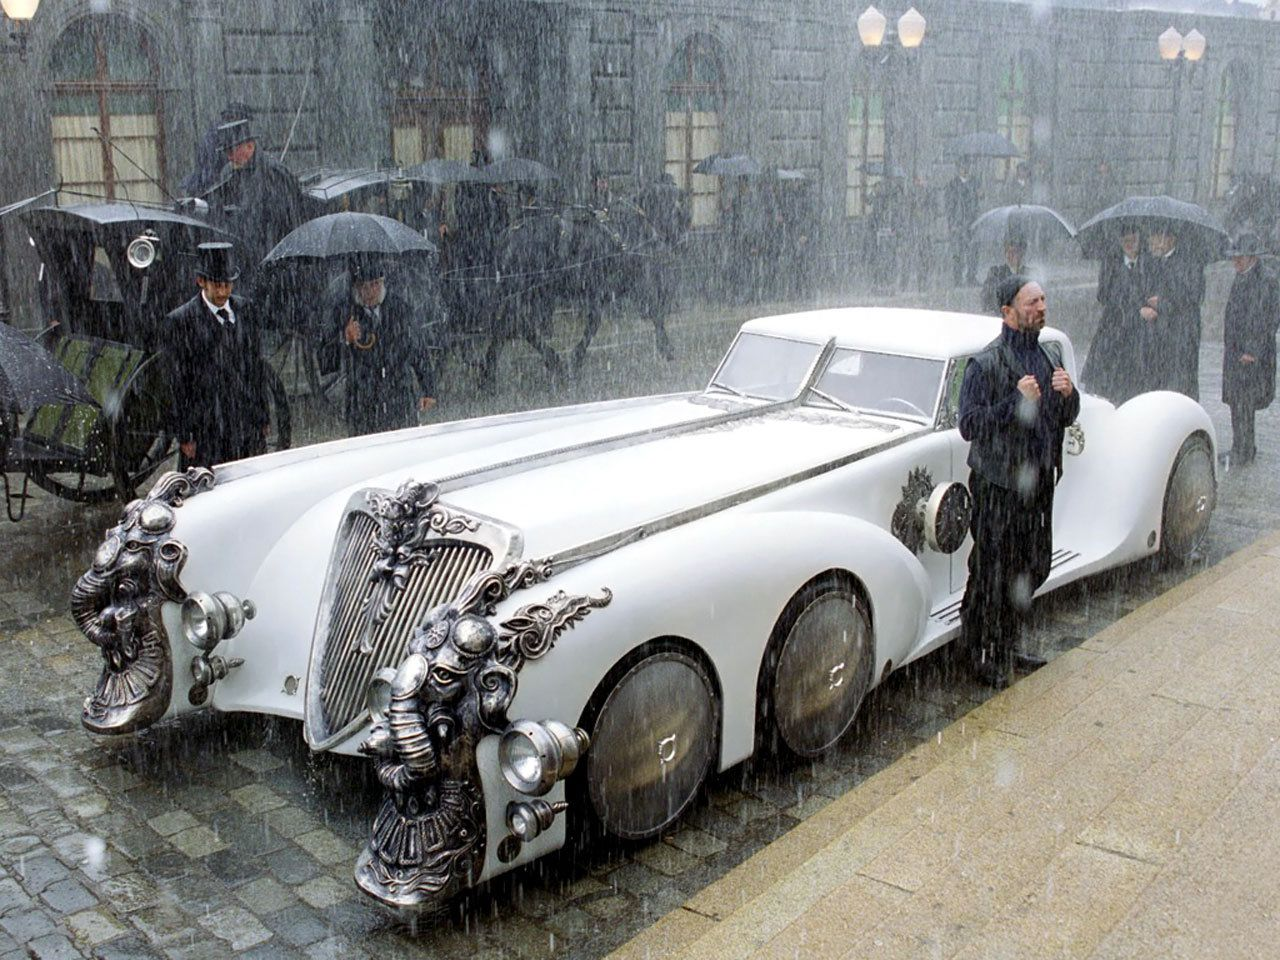
\includegraphics[height=6cm]{img/a_steampunk_car.jpg}
  \end{figure}
\end{frame}

\begin{frame}[c]{Modelisation, prospective et Steampunk ?}
  \vspace{-1cm}
  Revient à questionner le statut de l'un par rapport à l'autre
  \begin{figure}
    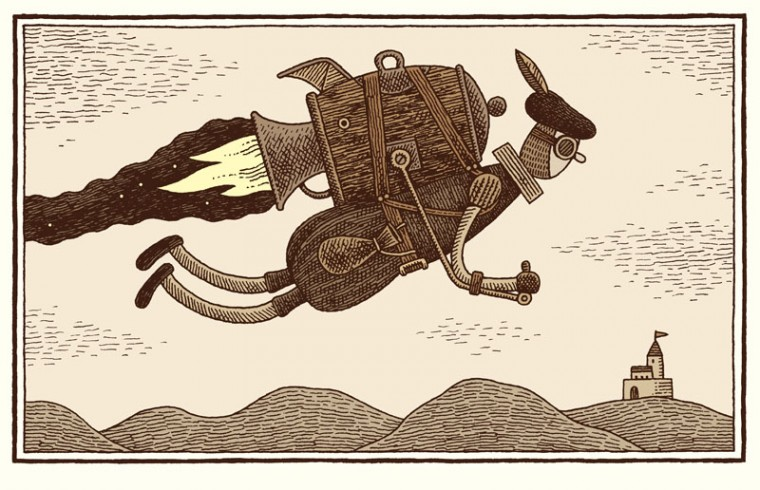
\includegraphics[height=6cm]{img/a_Tom-Gauld-jetpack.jpg}
  \end{figure}
\end{frame}

\begin{frame}[c]{Comment cela va-t-il se passer ?}
  \vspace{-1cm}
  \begin{itemize}
    \item Où se positionne le modèle
    \item Une rapide définition de la prospective territoriale
    \item Un exemple d'hybridation réussie ?
  \end{itemize}

  \begin{figure}
    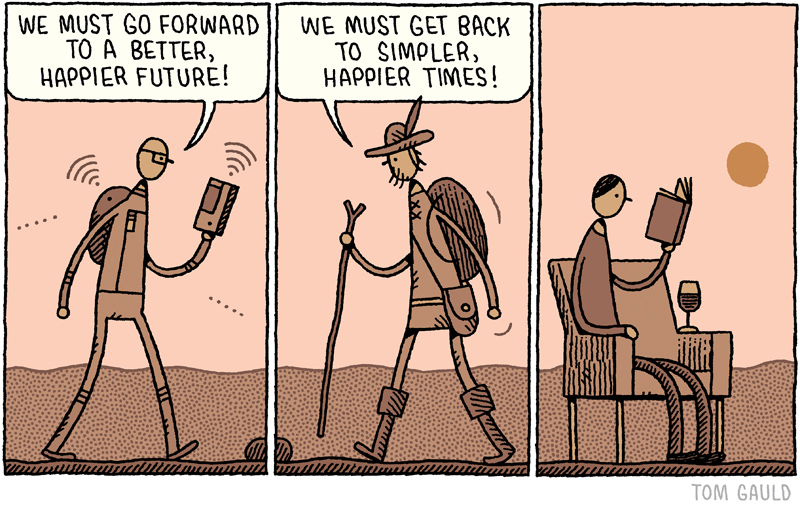
\includegraphics[height=4cm]{./img/a_Tom-Gauld-walk.jpg}
  \end{figure}
\end{frame}

\section{Epistemologie de la modelisation : le domaine}

%-=-=-=-=-=-=-=-=-=-=-=-=-=-=-=-=-=-=-=-=-=-=-=-=
%	FRAME: EPISTEMOLOGIE DE LA MODELISATION
%-=-=-=-=-=-=-=-=-=-=-=-=-=-=-=-=-=-=-=-=-=-=-=-=

\begin{frame}[c]{Du système au modèle, tentative de théorisation}
 \vspace{-1em}
  \begin{quote}
    <<le terme de \textbf{modèle} a la même signification que celui de concept ou d'hypothèse ou d'analogie [...], un modèle est une abstraction qui simplifie le système réel étudié [...] pour se focaliser sur les aspects qui intéressent le modélisateur et qui définissent les problématiques du modèle.>>
  \end{quote}
  \hspace*{\fill}\textsc{Coquillard et Hill 1997, p.7}
  \vspace{-0.5em}
  \begin{figure}
   	\centering
   		\subfigure{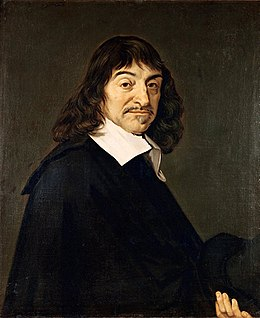
\includegraphics[height=3cm]{img/a_descartes.jpg}} \hspace{0.2em} %%descartes
      \subfigure{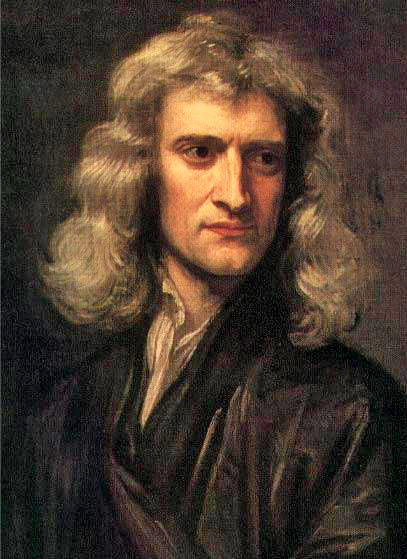
\includegraphics[height=3cm]{img/a_newton.jpg}} \hspace{0.2em} %% newton
   		\subfigure{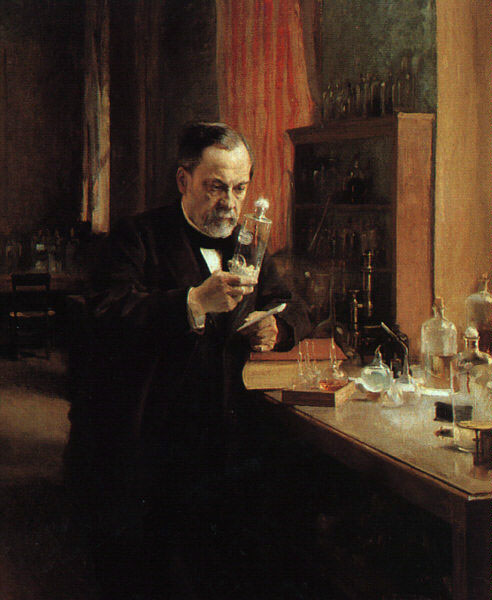
\includegraphics[height=3cm]{img/a_pasteur.jpg}} \hspace{0.2em} %%pasteur
      \subfigure{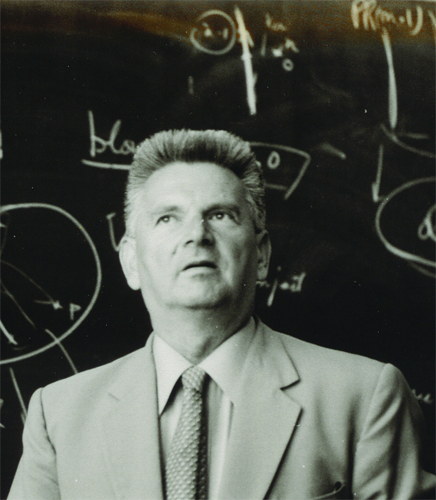
\includegraphics[height=3cm]{img/a_thom.png}} %%thom
  \end{figure}
\end{frame}

\begin{frame}[c]{Du système au modèle, tentative de théorisation}
  \vspace{-1em}
  \begin{quote}
    <<la \textbf{théorisation} [...] est liée à la possibilité de plonger le réel dans un virtuel imaginaire, doté de propriétés génératives, qui permettent de faire des prévisions.>>
  \end{quote}
  \hspace*{\fill}\textsc{Thom 2009, p. 91}
  \vspace{-0.5em}
  \begin{figure}
   	\centering
   		\subfigure{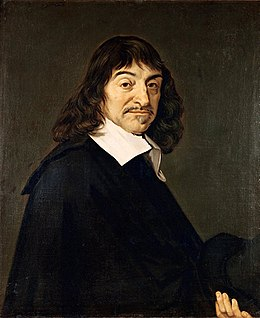
\includegraphics[height=3cm]{img/a_descartes.jpg}}\hspace{0.2em} %%descartes
      \subfigure{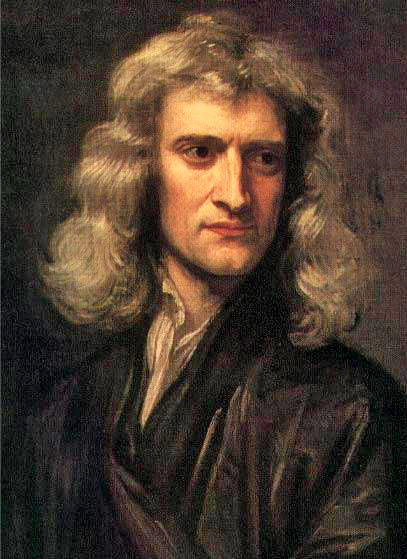
\includegraphics[height=3cm]{img/a_newton.jpg}}\hspace{0.2em} %% newton
   		\subfigure{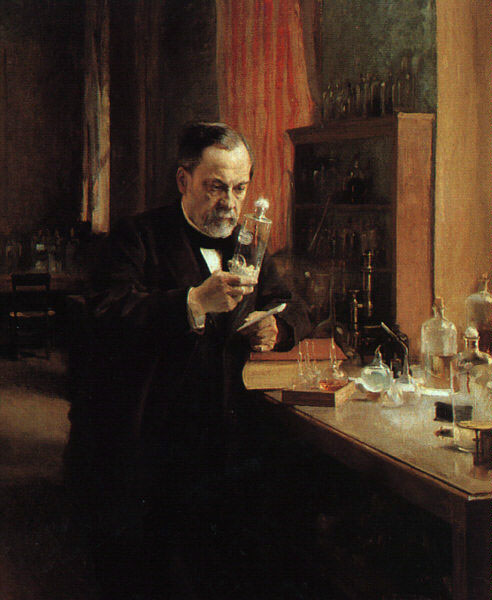
\includegraphics[height=3cm]{img/a_pasteur.jpg}}\hspace{0.2em} %%pasteur
      \subfigure{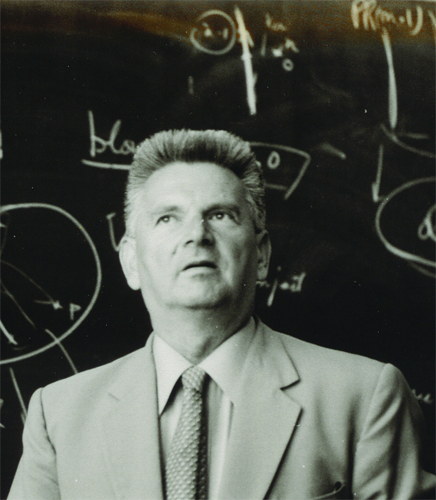
\includegraphics[height=3cm]{img/a_thom.png}} %%thom
  \end{figure}
\end{frame}

\begin{frame}[c]{Des modèles pour la recherche de formes}
  \vspace{-1em}
  \begin{quote}
    <<Peut-on, dans un paysage de phénomènes, reconnaître un objet ou une chose si l'on n'en a pas au préalable le concept ? C'est aussi simple que ça. \textbf{Si l'on n'a pas le concept d'un objet, on ne le reconnaîtra pas}. [...] La possibilité de reconnaître un être en général, une entité dans un paysage empirique, est toujours à mon avis subordonnée à une conceptualisation>>
  \end{quote}
  \hspace*{\fill}\textsc{Thom 2009, p.93}
  \vspace{-0.5em}
  \begin{figure}
   
\includegraphics[height=3cm]{img/a_rorschach.png}
  \end{figure}
\end{frame}

\section{Epistemologie de la\\ modelisation : simulation}
%-=-=-=-=-=-=-=-=-=-=-=-=-=-=-=-=-=-=-=-=-=-=-=-=
%	FRAME: CONTROVERSE
%-=-=-=-=-=-=-=-=-=-=-=-=-=-=-=-=-=-=-=-=-=-=-=-=

\begin{frame}[c]{Des modèles pour la recherche de formes}
  \vspace{-1em}
  \begin{quote}
    << La \textbf{simulation consiste à faire évoluer une abstraction d’un système au cours
    du temps} afin d’aider à comprendre le fonctionnement et le comportement de
    ce système et à appréhender certaines de ses caractéristiques dynamiques dans
    l’objectif d’évaluer différentes décisions.>>
  \end{quote}
  \hspace*{\fill}\textsc{Coquillard} et \textsc{Hill} (1997, p.11)
  \vspace{-0.5em}
  \begin{figure}
   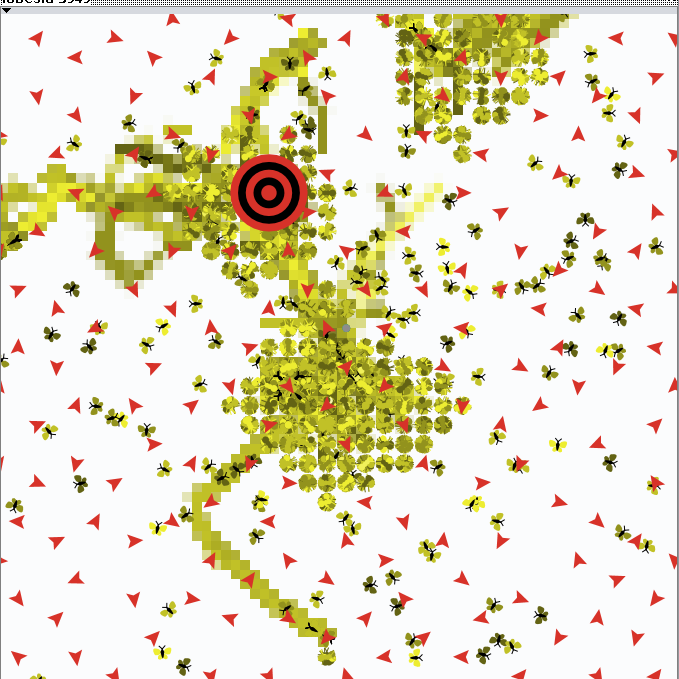
\includegraphics[height=3cm]{img/a_view_zoom_dist2.png}
  \end{figure}
\end{frame}


\begin{frame}[c]{Phylogénie des approches de simulation}
  \vspace{-2em}
  \begin{figure}
   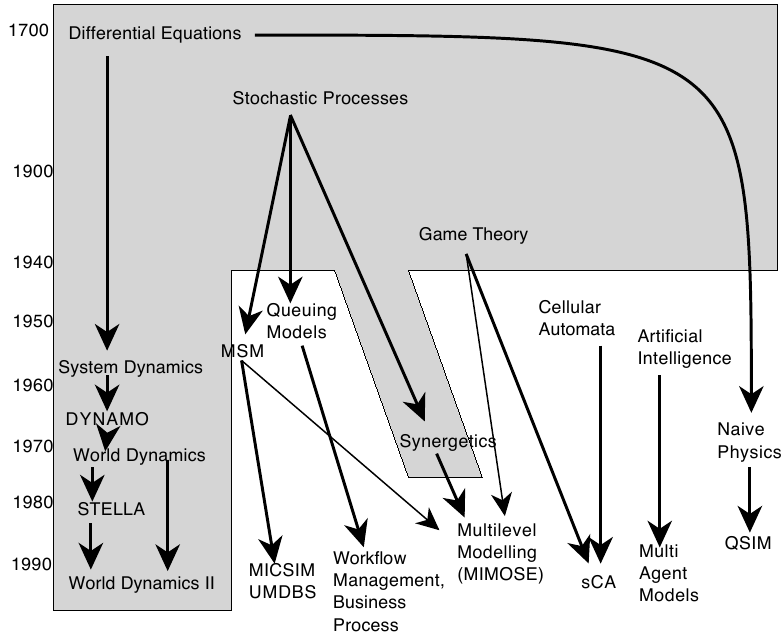
\includegraphics[height=6cm]{img/a_troitzsch_1997.png}
  \end{figure}
  \vspace{-0.8em}
  \small{Le développement de l'approche de simulation contemporaine en sciences sociales (d'après \textsc{Troitzsch} 1997). La partie grise représente les modèles à base d'équation, la partie blanche les modèles à base d'objets, d'événements, ou d'agents}.
\end{frame}

\begin{frame}[c]{modèles à base d’équation}
  \vspace{-2em}
  Désignent un ensemble diversifié de modèles mathématiques, algorithmes informatiques et méthodes statistiques qui ont pour objectif de reproduire des motifs de données empiriques.
  \begin{figure}
   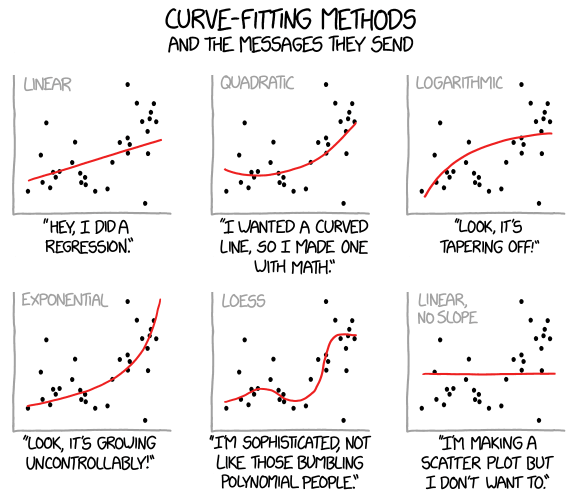
\includegraphics[height=6cm]{img/a_curve_fitting.png}
  \end{figure}

\end{frame}

\begin{frame}[c]{modèles à base d’objets/d’événements/d’agents}
  \vspace{-2em}
  Désignent un ensemble diversifié de modèles dans lesquels des entités entre en interactions. C'est de cette interaction que naît la complexité.
  \begin{figure}
   	\centering
   		\subfigure{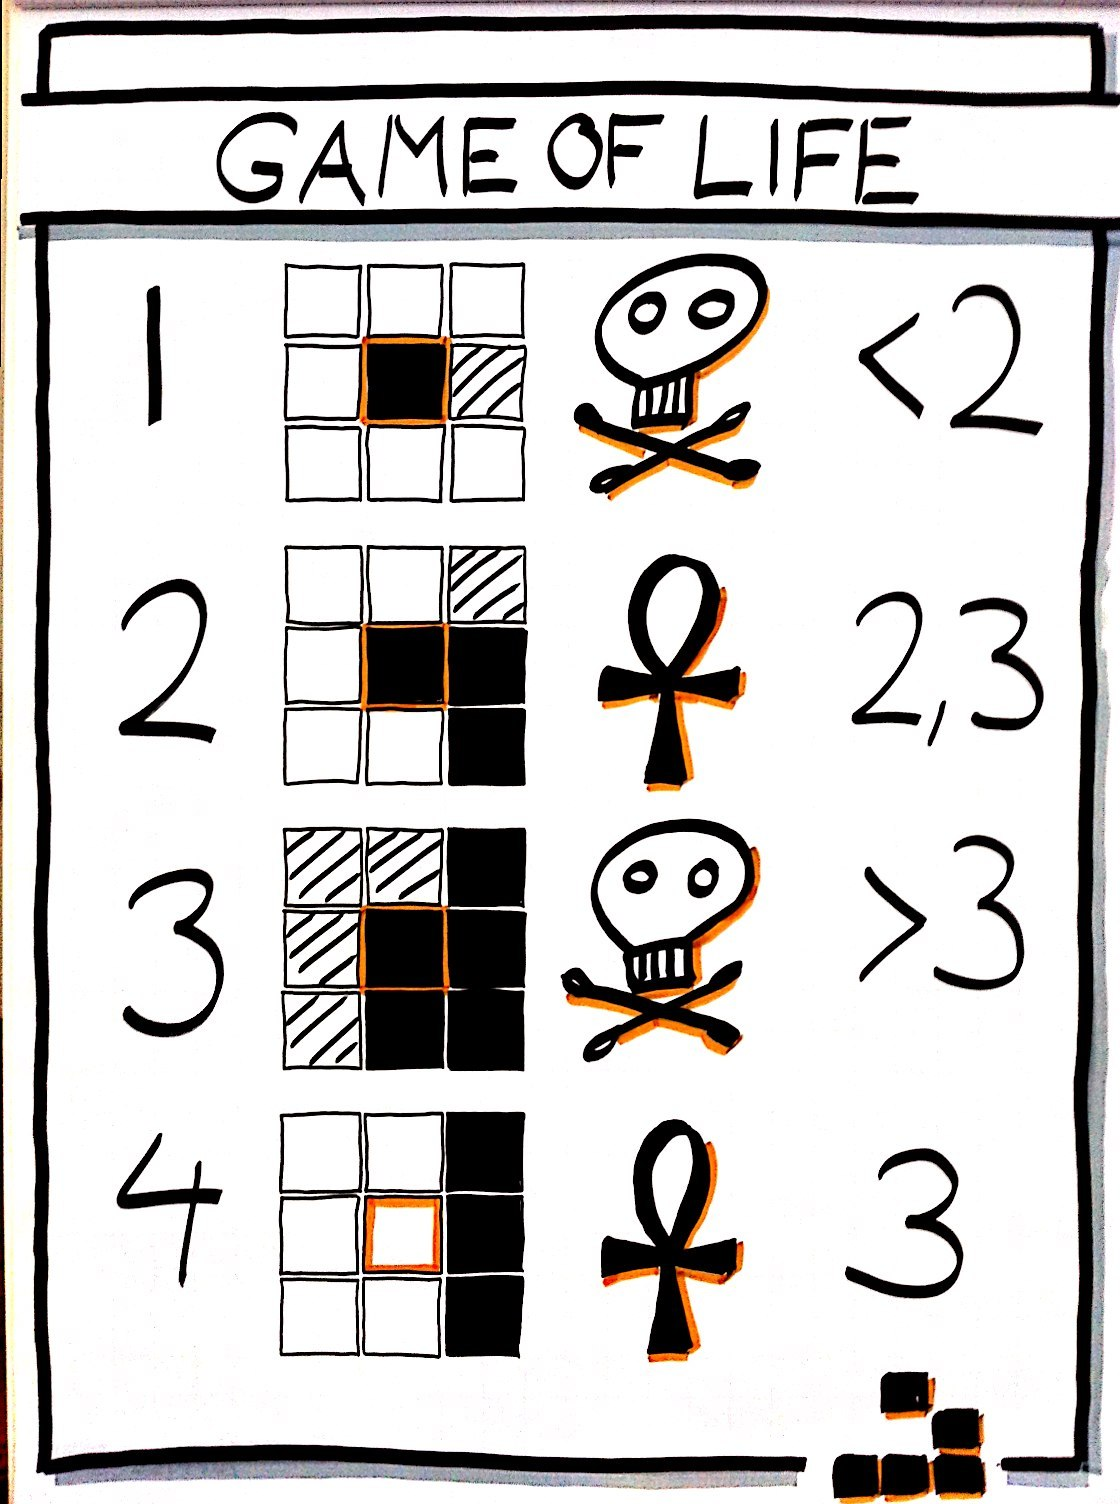
\includegraphics[height=6cm]{img/a_gameofliferules11.jpg}}\hspace{0.2em} %%xkcd
      \subfigure{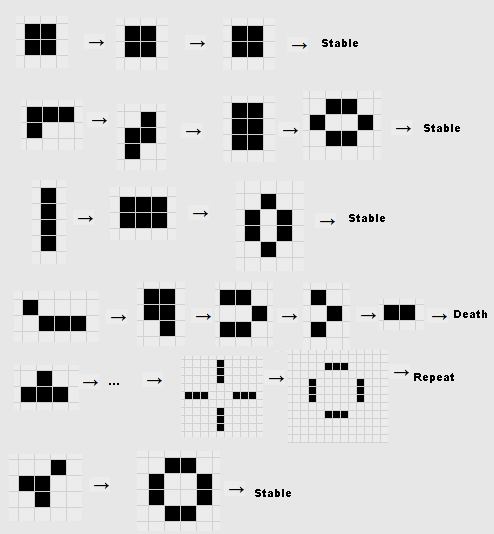
\includegraphics[height=6cm]{img/a_gameOfLife.png}}\hspace{0.2em} %% game of life
  \end{figure}

\end{frame}

\begin{frame}[c]{Les systèmes multi-agents}
  \vspace{-2em}
  \small
  \begin{quote}
    "[...] une entité physique ou virtuelle :
      \begin{itemize}
        \item qui est capable d'agir dans un environnement ;
        \item qui peut communiquer directement avec d'autres agents ;
        \item qui est mue par un ensemble de tendances;
        \item qui est capable de percevoir (mais de manière limitée) son environnement ;
        \item qui ne dispose que d'une représentation partielle de cet environnement (et éventuellement aucune) ;
        \item dont le comportement tend à satisfaire ses objectifs, en tenant compte des ressources et des compétences dont elle dispose, et en fonction de sa perception et des communications qu'elle reçoit".
      \end{itemize}
  \end{quote}
  \hspace*{\fill}\textsc{Ferber 1995, p.13}
\end{frame}

\begin{frame}[c]{KISS et KIDS}
  \vspace{-2em}
  \begin{itemize}
    \item KISS (\textit{Keep It Simple, Stupid!}) expliquer un phénomène observé $\rightarrow$ générer par simulation les microspécifications nécessaires et suffisantes pour reproduire le macrophénomène observé (Epstein et Axtell, 1996).
    \item KIDS (\textit{Keep It Descriptive, Stupid!}) : importance de conserver une approche explicative et de rendre toute ou partie des tâches isomorphes aux phénomènes observés (Edmonds et Moss 2005).
    \item {\color{lightgray}KILT (\textit{Keep It a Learning Tool!}) : Le page et Perroton (2017)}
  \end{itemize}
  \vspace{-1em}
  \begin{figure}
   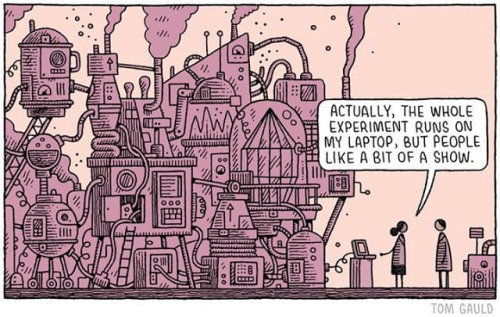
\includegraphics[height=3cm]{img/a_KIDS.jpg}
  \end{figure}
\end{frame}

\begin{frame}[c]{Pourquoi modéliser et simuler}
  \vspace{-2em}
  \begin{itemize}
    \item comprendre et formaliser un système réel
    \item calibrer ou optimiser un système simulé
    \item Explorer les réactions du modèle :
    \begin{itemize}
      \item analyse de sensibilité
      \item calibration à partir de motifs (\textit{pattern})
      \item Pattern Space Exploration : (output exploration)
    \end{itemize}
  \end{itemize}
  \vspace{-1em}
  \begin{figure}
   
\includegraphics[height=4cm]{img/a_gauld_nutts.jpg}
  \end{figure}
\end{frame}

%-=-=-=-=-=-=-=-=-=-=-=-=-=-=-=-=-=-=-=-=-=-=-=-=
%
%	SECTION: PROSPECTIVE
%
%-=-=-=-=-=-=-=-=-=-=-=-=-=-=-=-=-=-=-=-=-=-=-=-=
\section{La prospective}

\begin{frame}[c]{La prospective : au passé}
  \vspace{-2em}
  Issue du monde de l'entreprise au moment de la dissociation des responsabilités
  \begin{itemize}
    \item stratégiques (fixer les objectifs)
    \item tactiques (moyen pour y parvenir)
  \end{itemize}
  \textbf{Objectif} : Une vision à long terme pour ne pas se laisser perturber par les ajustements que nécessite la réalité.
  \begin{figure}
   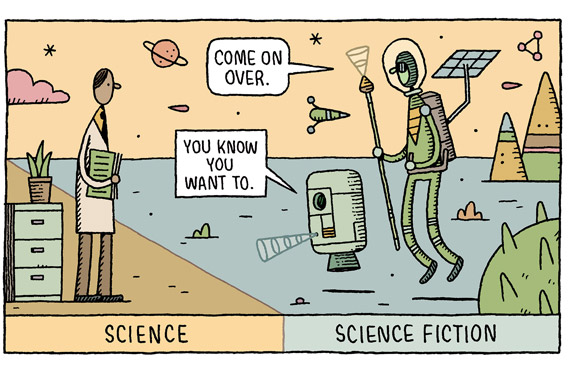
\includegraphics[height=4cm]{img/a_gauld_tom_new_scientist.jpg}
  \end{figure}
\end{frame}

\begin{frame}[c]{Sur les épaules des géants}
  \vspace{-2em}
  La prospective n'a d'intérêt qu'à partir du moment où les acteurs s'en saisissent pour mener à bien des projets sur le temps long. (\textsc{M. Sebillote, Aigrain}, \textit{et al.} 2003, p. 330)
  \begin{figure}
   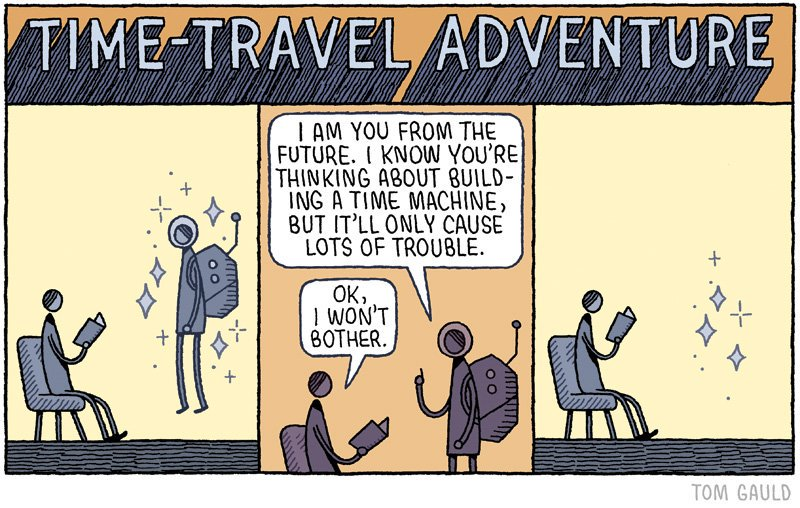
\includegraphics[height=4cm]{img/a_thom_gauld_futureMachine.jpg}
  \end{figure}
  \begin{quote}
    <<Ce n'est donc pas seulement le passé qui explique l'avenir, mais aussi l'image du futur qui s'imprime dans le présent>>
    \hspace*{\fill}\textsc{Godet} 1985 p.29
  \end{quote}
\end{frame}

\begin{frame}[c]{Problèmes pernicieux et sciences post-normales}
  \vspace{-2em}
  Une démarche prospective essaie d'anticiper les "problèmes pernicieux" :  difficile ou impossible à résoudre en raison d'exigences incomplètes, contradictoires et changeantes qui sont souvent difficiles à reconnaître (\textsc{Rittel} 1974).

  Le recours à la participation des parties-prenantes quand les processus sont complexes, les faits incertains, les valeurs discutées et les enjeux élevés (\textsc{Funtowics} et \textsc{Ravetz} 1993)

  \begin{figure}
   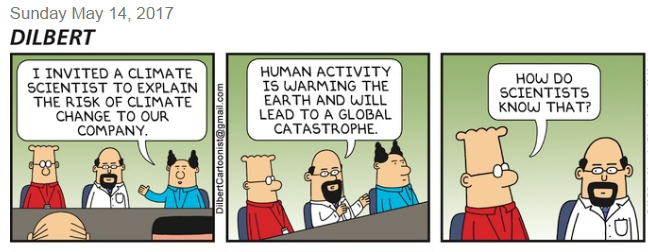
\includegraphics[height=4cm]{img/a_dilbert-climate-science.png}
  \end{figure}
\end{frame}

\begin{frame}[c]{Pourquoi simuler et prospectiver ?}
  \vspace{-2em}
  \begin{figure}
   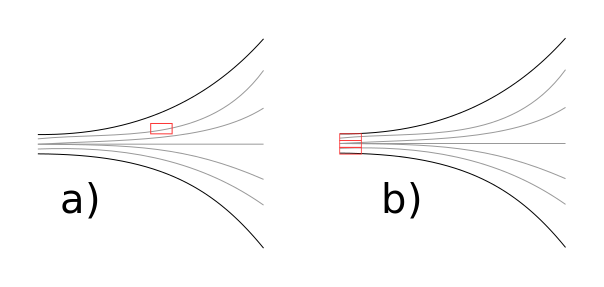
\includegraphics[height=5cm]{img/a_prospective_simulation.png}
  \end{figure}
  \vspace{-1em}
  \begin{quote}
    <<La simulation à base d’agents en sciences sociales : une "béquille pour l’esprit humain" >>
  \end{quote}
  \hspace*{\fill}\textsc{(Banos, 2010)}
\end{frame}
%-=-=-=-=-=-=-=-=-=-=-=-=-=-=-=-=-=-=-=-=-=-=-=-=
%
%	SECTION: HYBRIDATION, SMA COMMOD ET PROSPECTIVE
%
%-=-=-=-=-=-=-=-=-=-=-=-=-=-=-=-=-=-=-=-=-=-=-=-=
\section{Simulation et prospective : entrer dans le Steampunk ?}

\begin{frame}[c]{6 SMA bien ComMod}
  \vspace{-2em}
  \begin{itemize}
    \item Dion Still Alive {\color{lightgray}(\textsc{Delay} et \textsc{Chevallier} 2015)}
    \item Victor {\color{lightgray}(\textsc{Delay} et al, 2017)}
    \item Lame {\color{lightgray}(\textsc{Delay} et \textsc{Bourgoin}, 2012)}
    \item CiViSME {\color{lightgray}(\textsc{Delay} et al. 2015)}
    \item Acidity GIS {\color{lightgray}(\textsc{Delay} et al 2015)}
    \item CeLL {\color{lightgray}(\textsc{Delay} et \textsc{Caffarra}, 2016)}
  \end{itemize}
  \vspace{-2em}
  \begin{figure}
    \subfigure{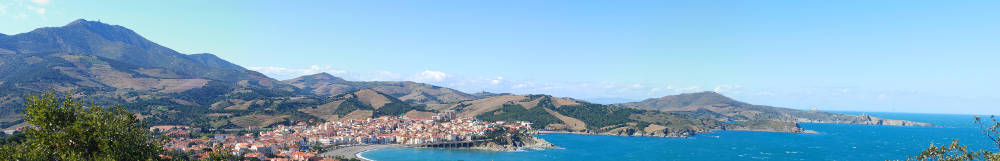
\includegraphics[height=1.5cm]{img/a_pano-banyuls.jpg}}\\ %%banyuls
     \subfigure{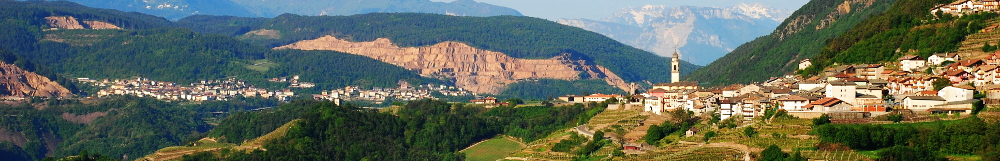
\includegraphics[height=1.5cm]{img/a_pano_cembra.jpg}} %% cembra
  \end{figure}
\end{frame}

\begin{frame}[c]{Mais ComMod c'est quoi?}
  \vspace{-2em}
  \begin{quote}
    << une posture scientifique de modélisation. Le processus de modélisation n'est rien d'autre qu'un objet intermédiaire qui facilite nos réflexions collectives et interdisciplinaires.>>
  \end{quote}
  \vspace{-2em}
  \begin{figure}
    \subfigure{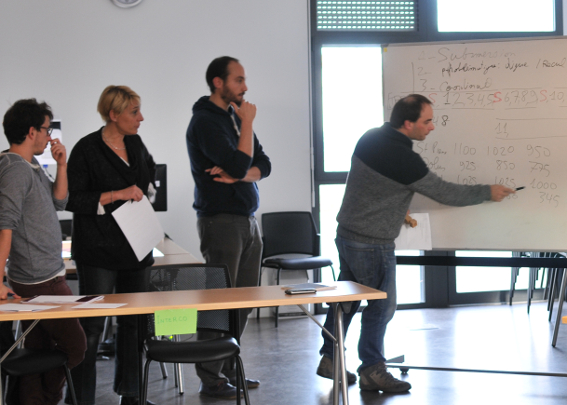
\includegraphics[height=2.5cm]{img/a_commod1}}\hspace{0.2em} %%banyuls
     \subfigure{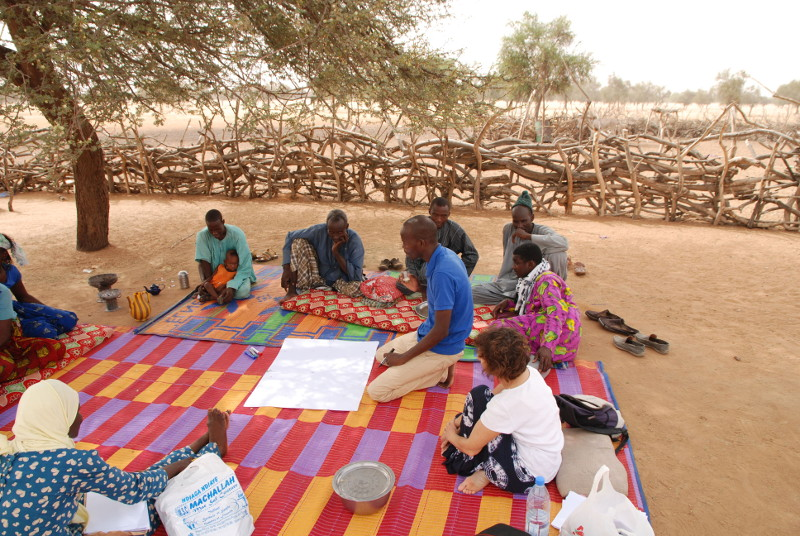
\includegraphics[height=2.5cm]{img/a_commod2}}\hspace{0.2em} %% cembra
     \subfigure{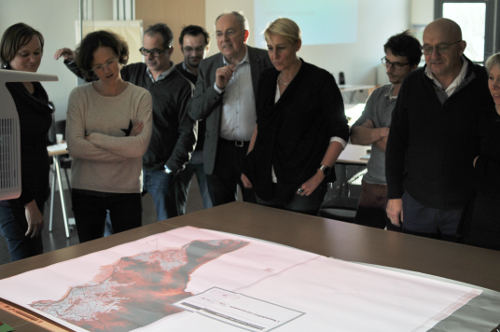
\includegraphics[height=2.5cm]{img/a_commod3}} %% cembra
  \end{figure}
\end{frame}

\begin{frame}[c]{Des SMA dans le fer à cheval}
  \vspace{-2em}
  \begin{figure}
   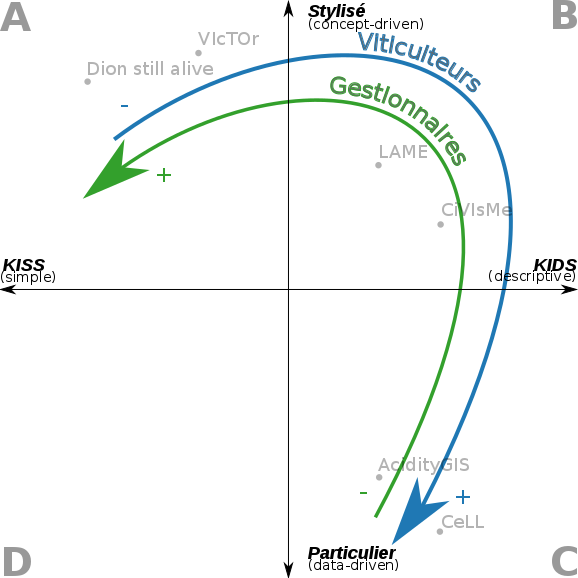
\includegraphics[height=6cm]{img/a_banos_sanders_positionnements.png}
  \end{figure}
  \hspace*{\fill}adapté de \textsc{Banos} et \textsc{Sanders} (2013)
\end{frame}

\begin{frame}[c]{Des modèles à la prospective}
  \vspace{-2em}
  \begin{figure}
   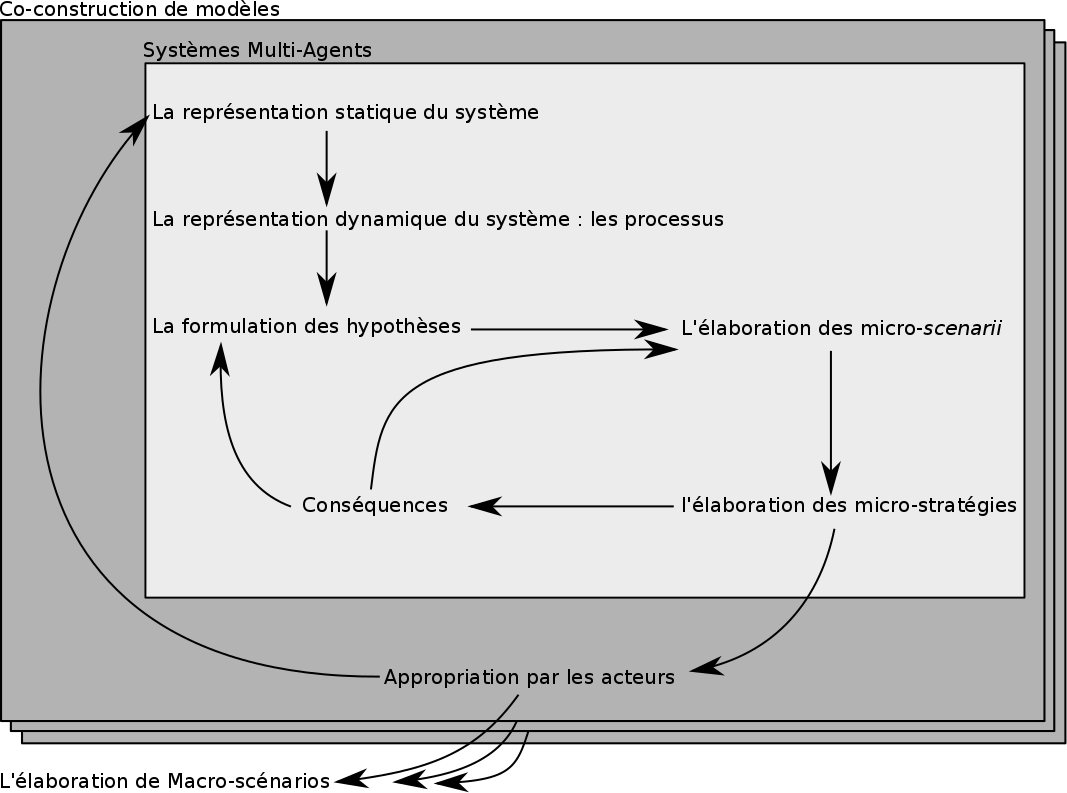
\includegraphics[height=6cm]{img/a_etapes_syspathmm.png}
   \caption{Les étapes de la démarche SYSPATHMM (\textsc{Sebillote et Sebillote,  2002})}
  \end{figure}
\end{frame}

\begin{frame}[c]{Des macro-variables}
  \vspace{-2em}
  11 macro-variables issues des modèles et validées en aveugle par les acteurs
  \begin{itemize}
    \item marché
    \item orographie
    \item qualité du produit
    \item incomes
    \item outcome
    \item prix du foncier
    \item structure sociale
    \item climat
    \item santé végétale
    \item évolution des règles d'échange
    \item évolution technique
  \end{itemize}
\end{frame}

\begin{frame}[c]{Un réseau d'interactions entre variables}
  \vspace{-2em}
  \begin{figure}
   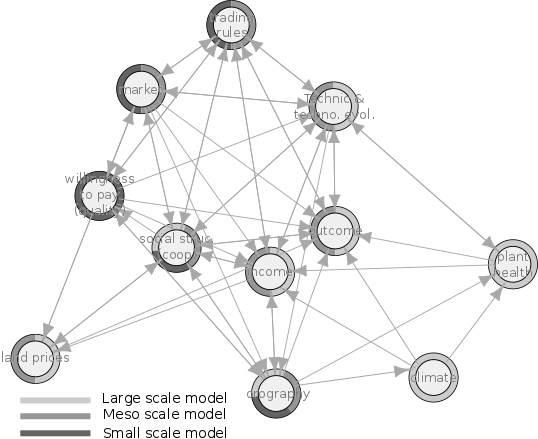
\includegraphics[height=6cm]{img/a_igraph_variables_structurelle.png}
   \caption{Relation entre les variables structurelles de la viticulture de forte pente}
  \end{figure}
\end{frame}

\begin{frame}[c]{Confronter les points de vue}
  \vspace{-2em}
  Utiliser le plan de motricité et de dépendance pour confronter la perception et la formalisation des variables qui agissent sur le territoire
  \begin{figure}
   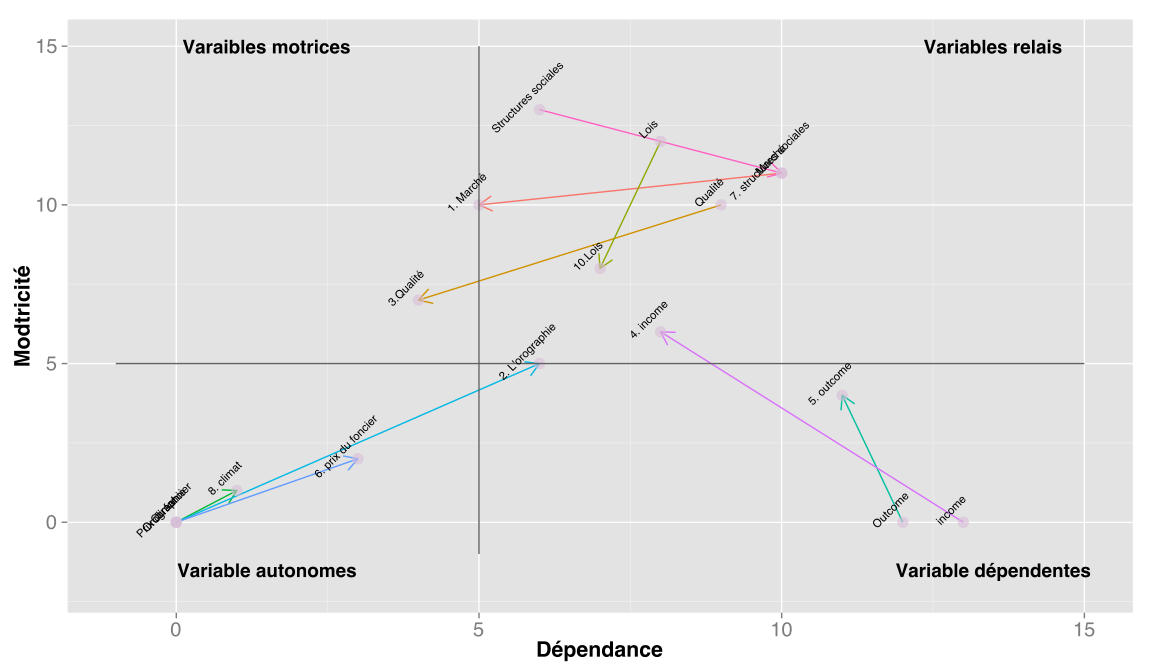
\includegraphics[height=6cm]{img/a_gg_plant_de_motricite_mvt.png}
  \end{figure}
\end{frame}


%-=-=-=-=-=-=-=-=-=-=-=-=-=-=-=-=-=-=-=-=-=-=-=-=
%
%	SECTION: CONCLUSION
%
%-=-=-=-=-=-=-=-=-=-=-=-=-=-=-=-=-=-=-=-=-=-=-=-=
\section{Conclusion}


\begin{frame}[c]{Ce qu'on veut retenir}
  \vspace{-2em}
  \begin{itemize}
    \item ComMod compatible avec la prise en compte l'incertitude
    \item Modèles à base d'agents pour modéliser l'imprévu (heuristique)
    \item La prospective pour enrichir l'heuristique
  \end{itemize}
  \begin{figure}
   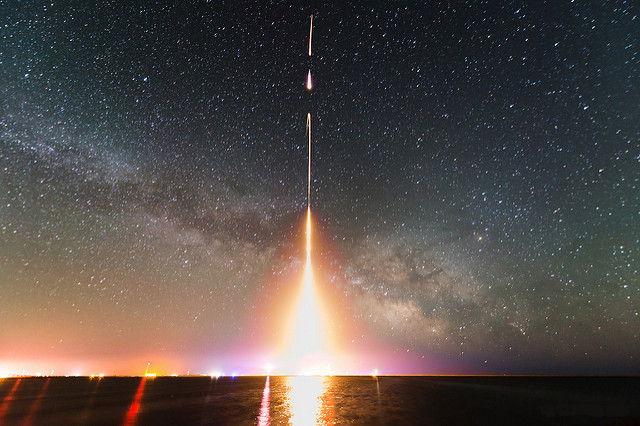
\includegraphics[height=6cm]{img/a_rocket.jpg}
  \end{figure}
\end{frame}

\begin{frame}[c]{Le drame de la solubilité}
  \vspace{-2em}
  \begin{itemize}
    \item Travailler au 21e Siècle avec des approches du 19e Sicèle (A.Reinhard, 2012).
    \item Veut-on que ce soit soluble dans le Steampunk ? (à quel prix ?)
    \begin{itemize}
      \item Comment l'éloigner de l'usine à gaz ?
    \end{itemize}
  \end{itemize}

  \begin{figure}
   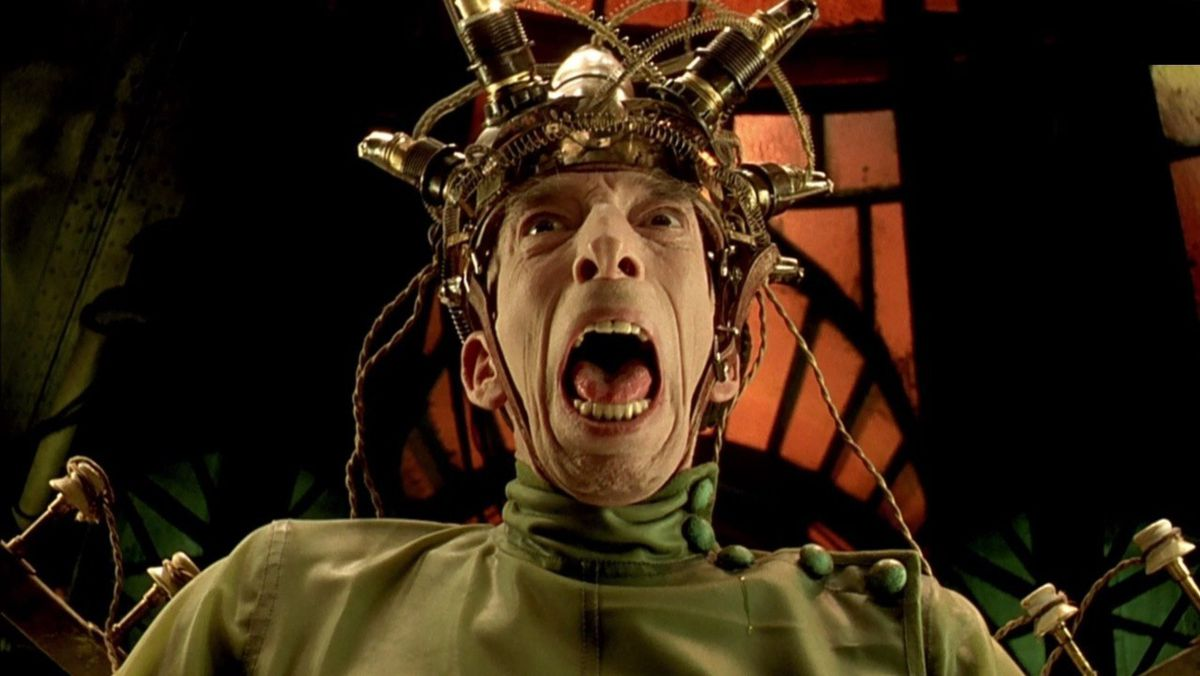
\includegraphics[height=5cm]{img/La_Cite_des_enfants_perdus.jpg}
  \end{figure}
\end{frame}

%-=-=-=-=-=-=-=-=-=-=-=-=-=-=-=-=-=-=-=-=-=-=-=-=
%
%	SECTION: Diapo final
%
%-=-=-=-=-=-=-=-=-=-=-=-=-=-=-=-=-=-=-=-=-=-=-=-=

{
%\usebackgroundtemplate{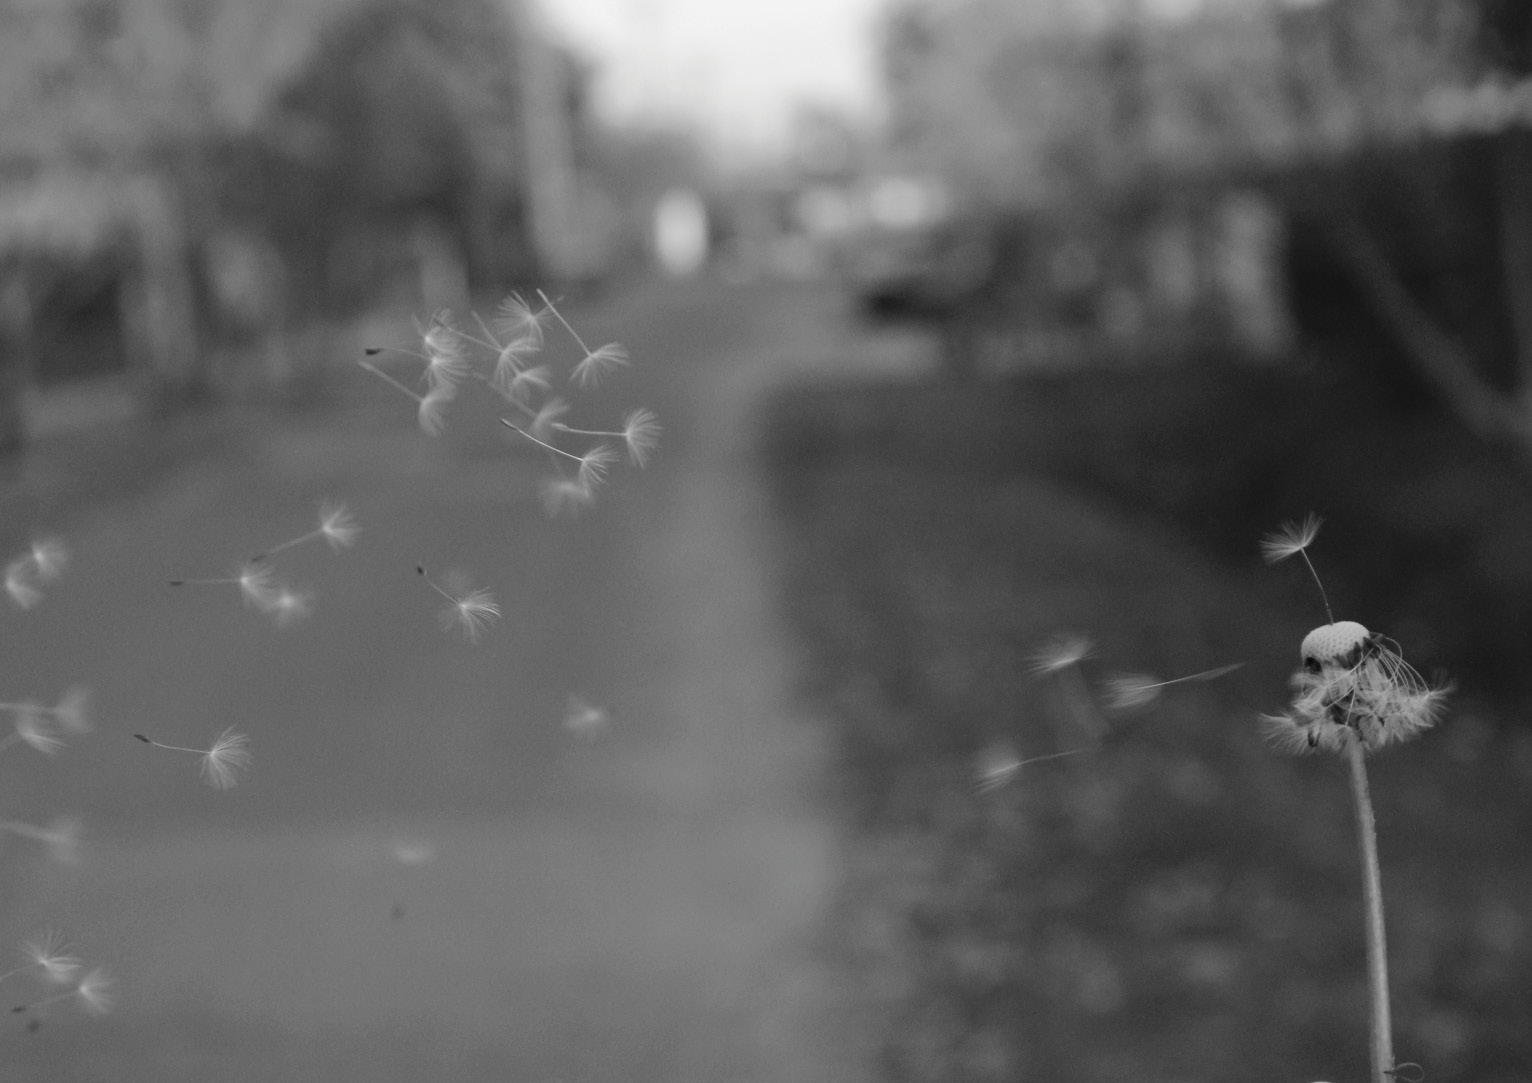
\includegraphics[width=1.05\paperwidth]{img/bw_fin.jpg}}%
\usebackgroundtemplate{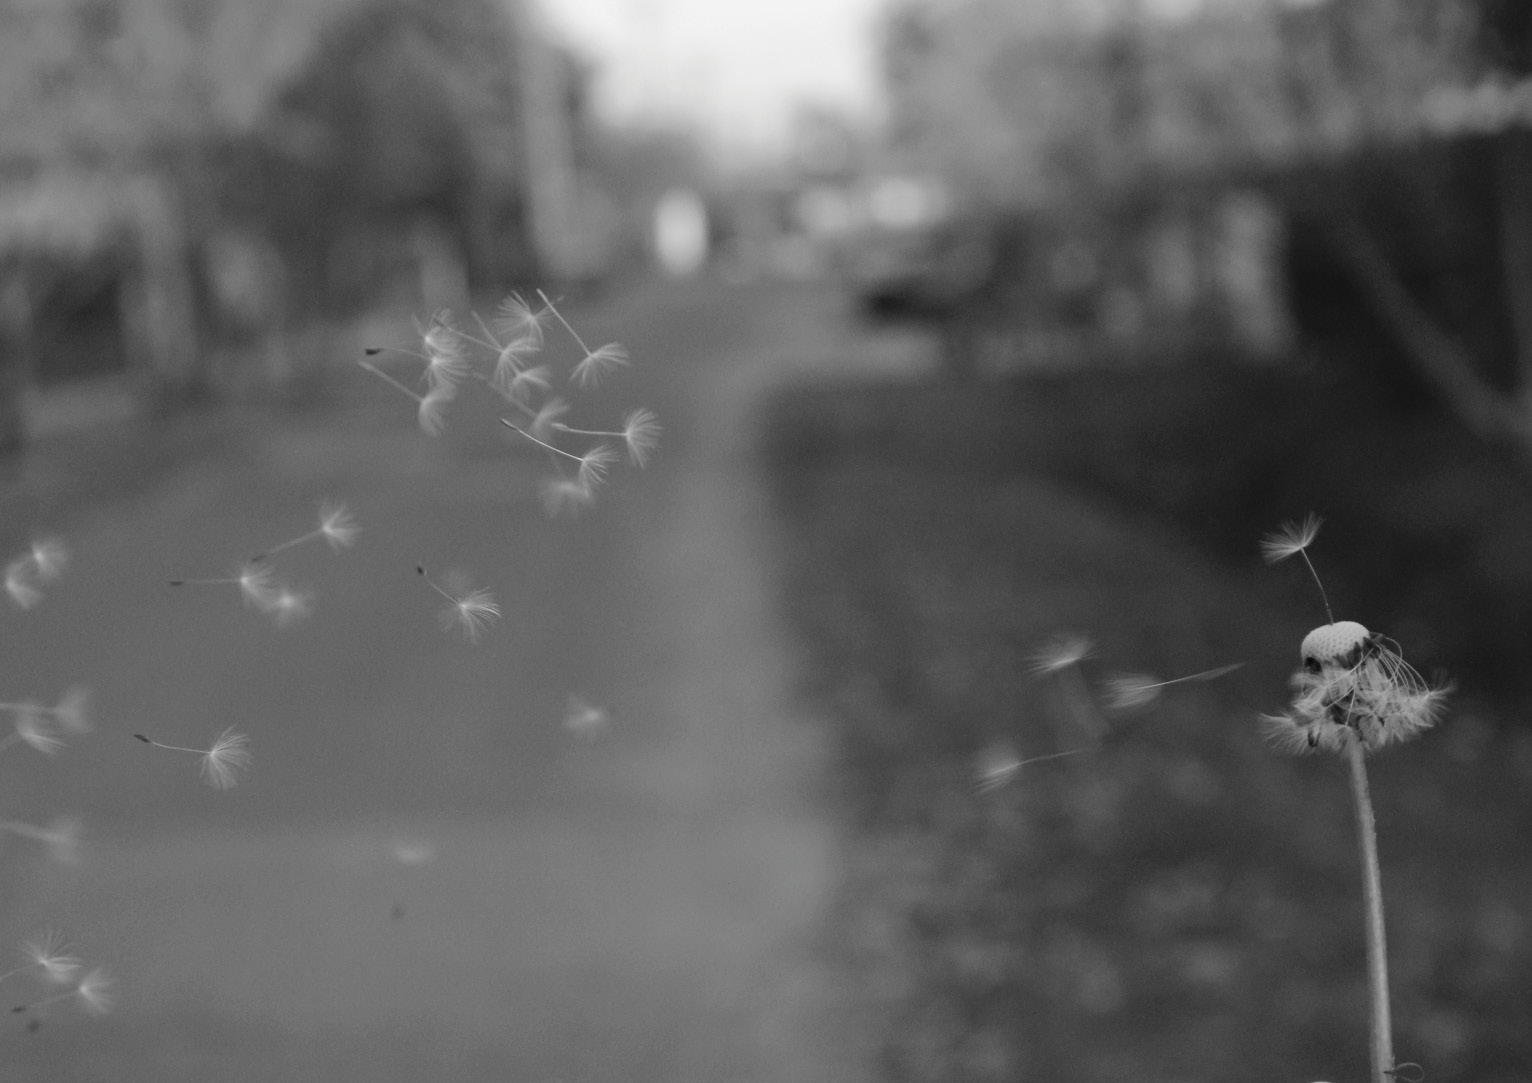
\includegraphics[width=1.05\paperwidth]{img/a_bw_fin.jpg}}%
\begin{frame}
  \begin{minipage}[t][.8\textheight]{\textwidth}
    %\color{\cnGrey}{\LARGE{Merci de votre attention}}

    \vfill

    \hfill \color{\cnGrey}{\LARGE{Merci de votre attention}}

    \hfill \small{Illustration : Thom Gauld, Scott Adams \& xkcd}
  \end{minipage}

\end{frame}
}

%%-=-=-=-=-=-=-=-=-=-=-=-=-=-=-=-=-=-=-=-=-=-=-=-=================
%%	FIN DU DIAPORAMA OFFICIEL
%%-=-=-=-=-=-=-=-=-=-=-=-=-=-=-=-=-=-=-=-=-=-=-=-=================

\end{document}
